\section{Introduction}\label{sec:intro}

\begin{figure*}
    \centering
    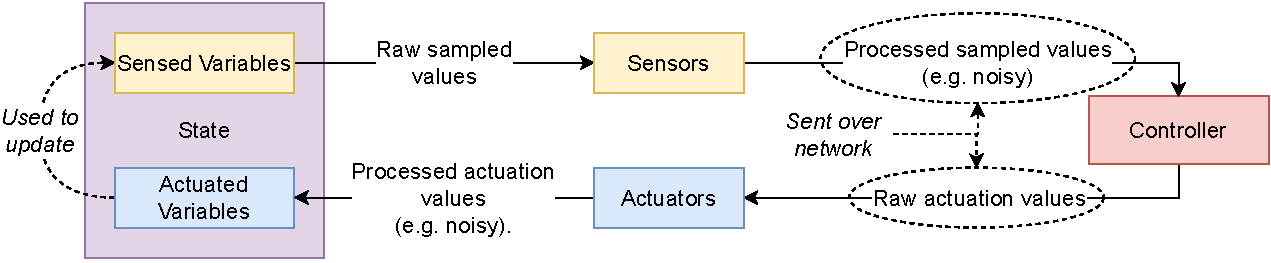
\includegraphics[width=.8\textwidth]{CLEAVE_NCS_structure}
    \caption{
        Structure of an emulated \acl*{NCS} in \acs*{CLEAVE}.
    }\label{fig:cleave:ncs:struct}
\end{figure*}

The number and applications of \acp{CPS}~\cite{Rajkumar2010CPS} --- i.e.\ systems in which a real, physical mechanism is controlled by a computer --- have exploded in recent years.
However, this rapid increase in adoption has mostly been limited to industrial contexts.
Although \acp{CPS} present huge opportunities for all facets of society, they have yet to reach our daily lives in any relevant scale due to their stringent operational requirements.
This is about to change, however, as with the advent of novel wireless communication technologies as well as networking paradigms, such as cellular 5G and edge computing~\cite{Satya2017Emergence}, consumer-grade \acp{CPS} will be made possible.
These technologies meet two key requirements of \acp{CPS}: real-time capabilities (through extremely low end-to-end latencies), and context- and locality-awareness, and will most likely become the backbone of \ac{CPS} in the future.

\acp{NCS}~\cite{Gupta2010NCSOverview}, a type of \ac{CPS} wherein multiple networked actuators and sensors form a part of the same automatic control system will benefit from the adoption of these technologies.
Depending on the physical system being controlled, \acp{NCS} can have stringent timing and reliability requirements for communication that conventional cloud paradigms and cellular networks can't meet\cite{Wan2020Efficient}.

\cite{Zhang2016Survey} is dedicated to the modelling and performance characterization of \acp{NCS}, improving NCSs by distributing control functions across networks, facilitating centralized coordination, control, and monitoring.

% Most of the literature concerning \acp{NCS}, follows a theoretical approach, and only a small fraction of it deals with experimental studies.
A number of works concerning \acp{NCS} deal with experimental studies.
\acp{NCS} have an inherently inter-domain nature intertwining knowledge from the fields of communications, computing, and control theory in ways that cannot be studied in isolation, leading to various different approaches to such studies.
One such approach uses setups in which the complete system is built on top of real hardware.
This approach is employed in the works of  \textcite{Baumann2018LowPower,Cuenca2019UAV}; in all of these, the authors implement their approach on physical testbeds.
Conversely, other studies choose to instead use completely \emph{simulated} \ac{NCS} setups. The authors in \cite{Ma2019DynamicSched} have opted for such a completely virtualized approach. These studies often employ combinations of physical and network simulation tools trying to capture the complex dynamics of \acp{NCS}.
Finally, some experimental studies instead employ \emph{virtualized} approaches, in which either
\begin{enumerate*}[itemjoin={{; }}, itemjoin*={{; or }}]
    \item a real network interacts with a simulated or emulated control system~\cite{Wang2020VoltageControl}
    \item a simulated network interacts with a real control system~\cite{Natale2004InvPendEthernet}.
\end{enumerate*}

As evidenced above, experimental research in \acp{NCS} includes varied heterogeneous hardware and software platforms, methodologies and \aclp*{KPI}.
This, in turn, leads to hardware, software, and methodology fragmentation, as different studies tend to prefer approaches more favored in their respective communities.

Furthermore, existing studies tend to focus on individual aspects and components of a system, thus producing results which do not provide a complete image of the \ac{NCS}.
This has caused a gap in knowledge pertaining to the reproducibility and comparison of experimental studies on these systems.

\textcite{Zoppi2020NCSBench} made the first (and to the best of our knowledge, the only) attempt at tackling this challenge in their work.
Their proposed platform \emph{NCSbench} is an open-source \ac{NCS} benchmarking platform, built utilizing LEGO\textregistered{}\ Mindstorms EV3 Core Set\texttrademark{}\ platform. It is reproducible because of its low-cost and accessibility. Although important for the reproducibility of \ac{NCS} benchmarks, we believe it is still inadequate given the reliance on specific hardware for the Plant which although flexible, limits the benchmarking to only those systems which can be physically implemented.
It is \emph{not} scalable, and thus unsuitable for distributed \acp{NCS}.

In this paper, we present the first fully-software-based framework for scalable and repeatable benchmarking of edge-native \ac{NCS}.
As edge computing begins being adopted by industry, more and more variations have begun to appear in literature.
``Near'', ``far'', ``core'', and ``telco'' edge describe variations of the original concept and are becoming ubiquitous in new research.
While the core idea of edge computing is widely accepted as fundamental for pervasive \acp{NCS} in general, understanding the strenghts and weaknesses of such different edge concepts is of paramount importance.

Our framework, \ac{CLEAVE}, aims to simplify the repeatable and scalable benchmarking of such systems.
It is fully virtualized, inspired by our previous work on benchmarking human-in-the-loop applications on the edge~\cite{Olguin2019EdgeDroid}.
The tool consists of a benchmarking framework and software development kit for the development of emulated physical systems and softwarized controllers.
These virtual \acp{NCS} can then be deployed on real networks for reparametrizable, repeatable, and reproducible benchmarking of the complete system.

\ac{CLEAVE} is built using \emph{Python 3.8}, making it highly extensible and able to harness the multitude of already existing user libraries.
It is furthermore compatible with container technologies such as \emph{Docker}\footnote{Docker Engine: \url{https://www.docker.com/}}, making it suitable for automated deployment, scaling, and benchmarking on industry-standard edge setups using container orchestration solutions.

The rest of this paper is structured as follows.
\cref{sec:approach} presents the design principles and implementation of the framework.
In \cref{sec:experiments}, we present a series of experiments which validate the utility, flexibility, and repeatability of \ac{CLEAVE}.
Finally, in \cref{sec:conclusion} we conclude this work.